\documentclass[11pt, a4paper, USenglish]{article} % change ``USenglish'' to ``norsk'' if applicable.

\usepackage{graphicx} % Provides the \includegraphics command.
\usepackage{hyperref} % Provides clickable links. Always load last, but before cleveref

\usepackage{amsmath}
\usepackage{amsfonts}
\usepackage{cancel}

\usepackage{svg}
\usepackage{adjustbox}
\usepackage{pdfpages}

\usepackage{float}
\usepackage{placeins} % Include the placeins package at the beginning of your document
\usepackage{subcaption} % Include the subcaption package at the beginning of your document
\usepackage{caption} % Include the caption package at the beginning of your document
\usepackage{tikz}
\usetikzlibrary{arrows,positioning}
\usepackage{circuitikz} % for circuit diagrams

\usepackage{listings} % Include the listings package
\usepackage{xcolor} % for setting colors

% Define the MATLAB style
\lstdefinestyle{MATLAB}{
    language=Matlab, % Use the MATLAB language
    frame=single, % Add a frame around the code
    breaklines=true, % Allow line breaks
    postbreak=\mbox{\textcolor{red}{$\hookrightarrow$}\space}, % Indicate line breaks with a red arrow
    numbers=left, % Line numbers on the left
    numberstyle=\tiny\color{gray}, % Line numbers are tiny and gray
    commentstyle=\color{green}, % Comments are green
    stringstyle=\color{purple}, % Strings are purple
    keywordstyle=\color{blue}, % Keywords are blue
    basicstyle=\ttfamily % Use the typewriter font
}

%% To easily include matlab code, I would recommend to have a look at this answer https://tex.stackexchange.com/a/158816 which has nice examples.

%% It uses: https://ctan.org/pkg/matlab-prettifier

\begin{document}

% Titlepage
\title{TTK4130 Modelling and simulation}
\author{Gutta på MS}
\date{\today}
\begin{titlepage}
    \maketitle
    \begin{center}
    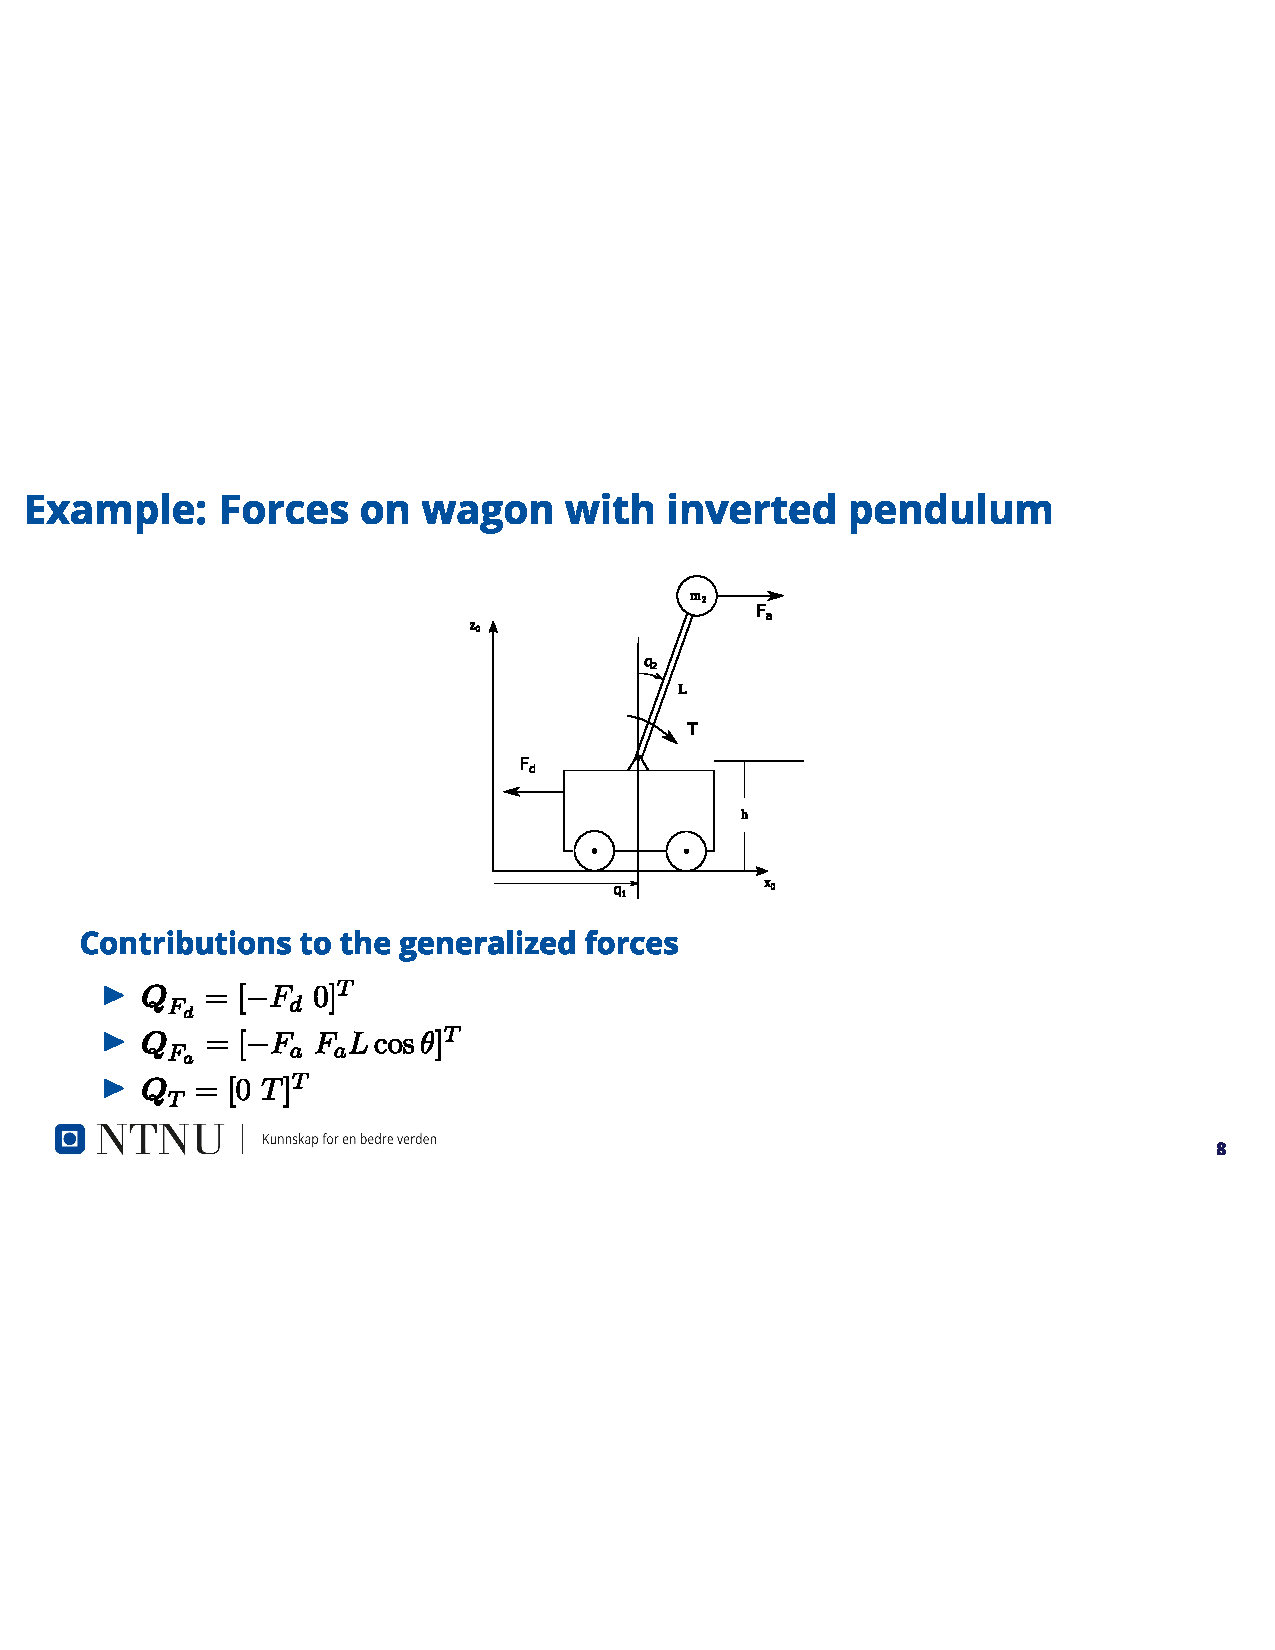
\includegraphics[scale=1, trim={7cm 12.5cm 7cm 9.4cm}, clip]{figures/wagon.pdf}
    \captionof*{figure}{\textit{Wagon with inverted pendulum}}
    \vfill % Add vertical space that expands to fill the available space
    
\includegraphics[scale=0.4]{figures/itk_ntnu}\\
    Department of Engineering Cybernetics
    \end{center}
    \thispagestyle{empty}
\end{titlepage}

% TOC
\newpage
\tableofcontents
\thispagestyle{empty} % Avoid page numbering on the table of contents.


% Main content
\newpage
\setcounter{page}{1}
\section{Kinematics}
\subsection{Vector notation}
There are two ways of expressing vectors:
\begin{subequations}
\begin{align}
    \mathbf{r}^i &= \begin{bmatrix} a \\ b \\ c \end{bmatrix} \\
    \vec{r}_{a/b} &= a\vec{i}_i + b\vec{j}_i + c\vec{k}_i
\end{align}
\end{subequations}
Where $i$ is the frame of reference, and subscript $a/b$ denotes from point b to point a. If the vectors are velocities, subscript $a/b$ denotes the velocity of point a relative to point b.
It is important to be consistent in the notation. Never do arithmetic operations on vectors expressed in different frames. This means: \newline
\begin{subequations}
\begin{align}
    \bcancel{\cancel{\vec{r}^i}}\\
    \bcancel{\cancel{\mathbf{v}^i+\mathbf{u}^a}}\\
    \bcancel{\cancel{\mathbf{v}^i \times \mathbf{u}^a}}
\end{align}
\end{subequations}

\subsection{Skew matrix notation}
If you have $\mathbf{u} = \begin{bmatrix}u_1 & u_2 & u_3\end{bmatrix}^\top$ and $\mathbf{v} = \begin{bmatrix}v_1 & v_2 & v_3\end{bmatrix}^\top$:
\begin{subequations}
    \begin{align}
    \mathbf{u}^\times = \begin{bmatrix}
                    0 & -u_3 & u_2 \\
                    u_3 & 0 & -u_1 \\
                    -u_2 & u_1 & 0
                  \end{bmatrix} \\
    \mathbf{u}^\times \mathbf{v} = \mathbf{u} \times \mathbf{v} \\
    \mathbf{u}^\times \mathbf{u} = 0 \\
    \left(\mathbf{u}^\times\right)^\times = -\mathbf{u}^\times \\
    \det{(\mathbf{u}^\times)} = 0  
    \end{align}
\end{subequations}
The cross product of two vectors can be calculated by finding the determinant of this matrix:
\begin{equation}
    \mathbf{u} \times \mathbf{v} = \det{\begin{bmatrix}
                    \vec{i} & \vec{j} & \vec{k} \\
                    u_1 & u_2 & u_3 \\
                    v_1 & v_2 & v_3
                  \end{bmatrix}}
\end{equation}

\subsection{Rotation matrices}
The rotation matrices are defined on each axis as:
\begin{subequations}
    \begin{align}
    \mathbf{R}_x(\theta) &= \begin{bmatrix} 1 & 0 & 0 \\ 0 & \cos(\theta) & -\sin(\theta) \\ 0 & \sin(\theta) & \cos(\theta) \end{bmatrix} \\
    \mathbf{R}_y(\phi) &= \begin{bmatrix} \cos(\phi) & 0 & \sin(\phi) \\ 0 & 1 & 0 \\ -\sin(\phi) & 0 & \cos(\phi) \end{bmatrix} \\
    \mathbf{R}_z(\psi) &= \begin{bmatrix} \cos(\psi) & -\sin(\psi) & 0 \\ \sin(\psi) & \cos(\psi) & 0 \\ 0 & 0 & 1 \end{bmatrix}
    \end{align}
\end{subequations}
Now lets say frame $a$ relative to frame $i$ is rotated by $\theta$ about the $x$-axis, $\phi$ about the $y$-axis, and $\psi$ about the $z$-axis. The rotation matrix from frame $a$ to frame $i$ is then:
\begin{equation}
    \mathbf{R}_i^a = \mathbf{R}_z(\psi)\mathbf{R}_y(\phi)\mathbf{R}_x(\theta)
\end{equation}
Which means that $\mathbf{R}_i^a$ is called the \textit{rotation matrix} from frame $a$ to frame $i$. Visually this is seen as moving the referance frame from $a$ to $i$, but it is used in transforming a vector from $i$ to $a$ (THE OPPOSITE ARG) for example: 
\begin{equation}
    \mathbf{v}_b = \mathbf{R}_i^b\mathbf{v}_i
\end{equation}
\begin{figure}[H]
    \centering
    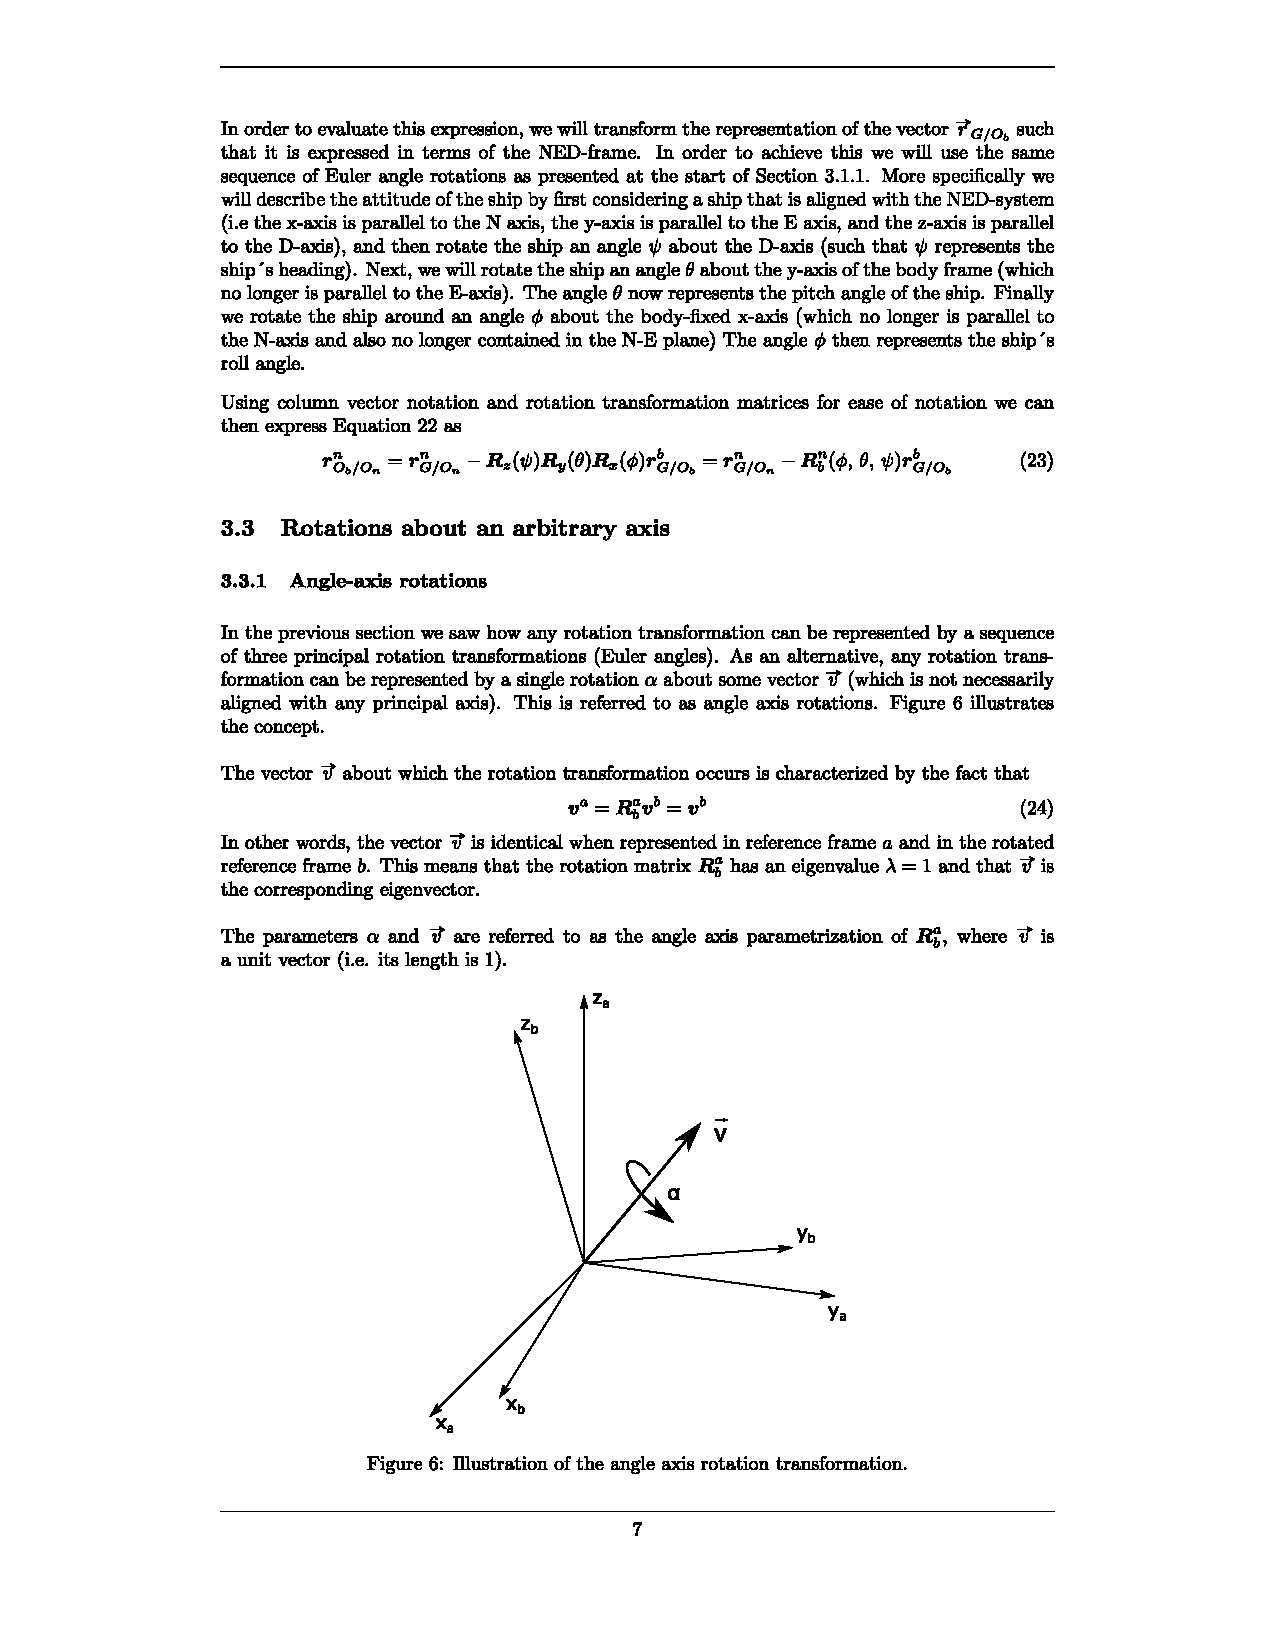
\includegraphics[scale=1, trim={7cm 3.5cm 7cm 16.5cm}, clip]{figures/arbitrary_axis_rotation.pdf}
    \caption{Rotation about arbitrary axis}
    \label{fig:arbitrary_axis_rotation}
\end{figure}
Now, if we have a rotation about an arbitrary axis $\mathbf{v}$, we can use the equation:
\begin{equation}
    \mathbf{R}_{\alpha,\vec{v}} = \cos(\alpha)\mathbf{I} + \mathbf{v}^\times\sin(\alpha) + \mathbf{vv}^\top(1-\cos(\alpha)) = \mathbf{R}_b^a(\alpha)
\end{equation}
\subsubsection{Properties of rotation matrices}
A couple of maybe interesting properties of rotation matrices:
\begin{subequations}
    \begin{align}
        \mathbf{v}^b=\mathbf{R}_a^b\mathbf{v}^a \\
        \mathbf{v}^a=\mathbf{R}_b^a\mathbf{v}^b \\
        \mathbf{R}_a^b\mathbf{R}_b^a = \mathbf{I} \\
        \mathbf{R}_a^b = \left(\mathbf{R}_b^a\right)^{-1} = \left(\mathbf{R}_b^a\right)^\top \\
        \dot{\mathbf{R}}_b^a = \left(\mathbf{\omega}_{ab}^a\right)^\times\mathbf{R}_b^a = \mathbf{R}_b^a\left(\mathbf{\omega}_{ab}^b\right)^\times \\
        \left(\vec{\omega}_{ab}^a\right)^\times = \dot{\mathbf{R}}_b^a\left(\mathbf{R}_b^a\right)^\top \\
        \vec{\omega}_{ad} = \vec{\omega}_{ab} + \vec{\omega}_{bc} + \vec{\omega}_{cd}
    \end{align}
\end{subequations}
Where the vector $\vec{\omega}_{ab}^a$ is the angular velocity vector from frame \textit{b} relative to frame \textit{b} with respect to frame \textit{a}.

\subsection{Linear and Angular Velocities and Acceleration in Different Frames}

Let \( \{0\} \) be the reference frame with coordinates \( x_0, y_0, z_0 \) and \( \{b\} \) be the body frame with coordinates \( x_b, y_b, z_b \). 

\subsection{Linear Velocity}

The linear velocity \( \vec{v}_{p/0} \) of a point \( p \) in the body frame \( \{b\} \) relative to the reference frame \( \{0\} \) is given by:

\[
\vec{v}_{p/0} = \vec{v}_0 + \vec{\omega}_{b/0} \times \vec{r}_{p/b}
\]

where:
\begin{itemize}
    \item \( \vec{v}_{p/0} \) is the linear velocity of point \( p \) in frame \( \{b\} \) relative to frame \( \{0\} \).
    \item \( \vec{v}_0 \) is the linear velocity of the origin of frame.
    \item \( \vec{\omega}_{b/0} \) is the angular velocity of frame \( \{b\} \) relative to frame \( \{0\} \).
    \item \( \vec{r}_{p/b} \) is the position vector of point p relative to the body frame \( \{b\} \).
\end{itemize}

\subsection{Linear Velocity with Time-Dependent Point \( p \)}

If the point \( p \) is a function of time, the linear velocity \( \vec{v}_{p/0} \) of a point \( p \) in the body frame \( \{b\} \) relative to the reference frame \( \{0\} \) is given by:

\[
\vec{v}_{p/0} = \vec{v}_{b/0} + \vec{\omega}_{b/0} \times \vec{r}_{p/b} + \vec{v}_{p/b}
\]

where \( \vec{v}_{p/b} \) is the velocity of point \( p \) relative to the body frame \( \{b\} \), given by:

\[
\vec{v}_{p/b} = \dot{p}_x \vec{i}_b + \dot{p}_y \vec{j}_b + \dot{p}_z \vec{k}_b
\]

Here, \( \dot{p}_x, \dot{p}_y, \dot{p}_z \) are the time derivatives of the coordinates of point \( p \) in the body frame.


\begin{itemize}
    \item \textbf{Linear Velocity}: Linear velocity can be thought of as the speed and direction at which a point on the body is moving relative to the fixed reference frame. It combines the translational movement of the entire body (described by \( \vec{v}_0 \)) with the rotational effect (described by \( \vec{\omega}_{b/0} \times \vec{r}_{p/b} \)).
    
\end{itemize}
\begin{itemize}
    \item \textbf{Alternative approach}
    This can also just be found by finding a the function for the point p in the zero frame ie:  (\( \vec{r}_{p/0} \)) and derivating this with respect to time. Remebering the importance of the chain rule this becomes equivalent and easy to solve on a beast calculator. (contact 41401071 for good price on beast calculator)
\end{itemize}

\subsection{Angular Velocity}

The angular velocity \( \vec{\omega}_{p} \) of point \( p \) is given by the sum of all contributing angular velocities:

\[
\vec{\omega_{p}} = \sum_{i} \omega_i \vec{e}_i
\]

where \( \omega_i \) are the individual angular velocity components about their respective principal axes \( \vec{e}_i \), representing the axis of rotation (it could be along $x_b$, $y_b$, or $z_b$).

\begin{itemize}
     \item \textbf{Angular Velocity}: Angular velocity describes how quickly and about which axis the body is rotating. The vector \( \vec{\omega}_{b/0} \) points along the axis of rotation \( \vec{e}_i \), and its magnitude \( \dot{\omega} \) indicates the rate of rotation.
\end{itemize}

\subsection{Angular Acceleration}

The angular acceleration \( \vec{\alpha}_{p} \) of point \( p \) is given by:

\[
\vec{\alpha_{p}} = \sum_{i} \dot{\omega}_i \vec{e}_i + \omega_i (\vec{\Omega}_i \times \vec{e}_i)
\]

where:
\begin{itemize}
    \item \( \dot{\omega}_i \) is the time derivative of the angular velocity component \( \omega_i \).
    \item \( \vec{\Omega}_i \) is the angular velocity of the reference frame of \( \mathbf{e}_i \).
    \item \( \vec{e}_i \) are the principal axes of the reference frame.
\end{itemize}

\subsection{Linear Acceleration}

The linear acceleration \( \vec{a}_{p/0} \) of point \( p \) relative to the reference frame \( \{0\} \) is given by:

\[
\vec{a}_{p/0} = \vec{a}_{b/0} + \vec{a}_{p/b} + \vec{\alpha}_{b/0} \times \vec{r}_{p/b} + \vec{\omega}_{b/0} \times (\vec{\omega}_{b/0} \times \vec{r}_{p/b}) + 2 \vec{\omega}_{b/0} \times \vec{v}_{p/b}
\]

where:
\begin{itemize}
    \item \( \vec{a}_{b/0} \) is the acceleration of the origin of the body frame \( \{b\} \) relative to the reference frame \( \{0\} \).
    \item \( \vec{a}_{p/b} \) is the acceleration of point \( p \) relative to the body frame \( \{b\} \).
    \item \( \vec{\alpha}_{b/0} \) is the angular acceleration of the body frame \( \{b\} \) relative to the reference frame \( \{0\} \).
    \item \( \vec{\omega}_{b/0} \) is the angular velocity of the body frame \( \{b\} \) relative to the reference frame \( \{0\} \).
    \item \( \vec{r}_{p/b} \) is the position vector of point p relative to the body frame \( \{b\} \).
\end{itemize}

\subsection{Explanation of Acceleration Components}

\begin{itemize}
    \item \textbf{Acceleration of Origin of Body Frame} (\( \vec{a}_{b/0} \)): This term represents the linear acceleration of the origin of the body frame \( \{b\} \) relative to the reference frame \( \{0\} \).
    \item \textbf{Acceleration of Point within Body Frame} (\( \vec{a}_{p/b} \)): This term represents the linear acceleration of point \( p \) within the body frame \( \{b\} \).
    \item \textbf{Linear Acceleration due to Angular Acceleration} (\( \vec{\alpha}_{b/0} \times \vec{r}_{p/b} \)): This term accounts for the linear acceleration of point \( p \) due to the angular acceleration of the body frame \( \{b\} \).
    \item \textbf{Centripetal Acceleration} (\( \vec{\omega}_{b/0} \times (\vec{\omega}_{b/0} \times \vec{r}_{p/b}) \)): This term represents the centripetal acceleration, which is the acceleration of point \( p \) due to its rotational motion about the origin of the body frame \( \{b\} \).
    \item \textbf{Coriolis Acceleration} (\( 2 \vec{\omega}_{b/0} \times \vec{v}_{p/b} \)): This term represents the Coriolis acceleration, which arises when point \( p \) is moving within the rotating body frame \( \{b\} \).
\end{itemize}



\subsection{Other stuff that might be usefull}
\textbf{Linear momentum} does not depend upn its point of reference:
\begin{subequations}
    \begin{align}
        \vec{p} = m\vec{v} \\
        \dot{\vec{p}} = m\vec{a} = \vec{F}
    \end{align}
\end{subequations}
\textbf{Angular momentum} of point \textit{p} with respect t origin \textit{o}, where $\vec{r}_{p/o}$ is the position of \textit{p} and $\vec{p}$ is the linear momentum. (Angular momentum depends upon its point of reference):
\begin{subequations}
    \begin{align}
        \vec{h}_{p/o} = \vec{r}_{p/o} \times \vec{p} \\
        \dot{\vec{h}}_{p/o} = \vec{r}_{p/o} \times \dot{\vec{p}} = \vec{T}
    \end{align}
\end{subequations}
\section{Newton-Euler Modelling}
Okay, your task is to model a system using Newton-Euler. Interesting, in my opinion the hardest of the three methods. But, let's get started.\newline
The Newton-Euler equations referenced to the center of mass in an inertial frame are given by:
\begin{equation}
    \mathbf{F}_{bc} = m \mathbf{a}_c
\end{equation}
\begin{equation}
    \mathbf{T}_{bc} = \mathbf{M}_{b/c} \cdot \boldsymbol{\alpha}_{ib} + \boldsymbol{\omega}_{ib} \times \left( \mathbf{M}_{b/c} \cdot \boldsymbol{\omega}_{ib} \right)
\end{equation}
\textbf{More complicated equations: } \newline
We use this when the forces and torques are not applied at the center of mass. The equations are given by:
The total torque acting in a arbitrary point P is given by:
\begin{equation}
    \vec{F}_{bo} = m \vec{a}_c
\end{equation}
\begin{equation}
    \mathbf{T}_{p} = \vec{r}_{c/p} \times m \vec{a}_c \cdot \mathbf{M}_{b/c} \cdot \boldsymbol{\alpha}_{ib} + \boldsymbol{\omega}_{ib} \times \left( \mathbf{M}_{b/c} \cdot \boldsymbol{\omega}_{ib} \right)
\end{equation}   
\textbf{Even more complicated equations: } \newline
If we apply newton euler equations in a non inertial frame, we get the following equations:
Non inertial frame means that the frame is accelerating. The equations are given by:
(børge wont do us like this though??)(this comes from setting up the equations of motion in a non inertial frame and then transforming them to the inertial frame with a rotation matrix)
\begin{equation}
    m \dot{\vec{v}}_c^a + m \vec{\omega}_ai^a \times \vec{v}_c^a = \vec{F}_{ac}^{a}
\end{equation}


\section{Rigid body, i have a rigid body ahhhh}
A \textbf{rigid body}; the distances between any two points within the body remain constant regardless of the external forces and torques applied to it.
\\
\\
\textbf{Degrees of Freedom:} A rigid body in three-dimensional space has six degrees of freedom: three translational (movement along the x, y, and z axes) and three rotational (rotation about the x, y, and z axes).

\subsection{Translational Motion (Newton's Second Law)}
\[
\vec{F}_{\text{ext}} = m \vec{a}_{\text{cm}}
\]

\subsection{Rotational Motion (Euler's Equations)}

The rotational motion of the rigid body is described by Euler's equations, which relate the rate of change of angular momentum to the external moments (torques) acting on the body. These equations are given by:

\[
\vec{T}_{\text{ext}} = \frac{d \vec{H}}{dt} + \vec{\omega} \times \vec{H}
\]

where:
\begin{itemize}
    \item \( \vec{T}_{\text{ext}} \) is the resultant external moment (torque) acting on the body.
    \item \( \vec{H} = \mathbf{J} \vec{\omega} \) is the angular momentum of the body.
    \item \( \mathbf{J} \) is the inertia tensor of the body.
    \item \( \vec{\omega} \) is the angular velocity of the body.
    \item \( \frac{d \vec{H}}{dt} \) is the time derivative of the angular momentum.
    \item \( \vec{\omega} \times \vec{H} \) is the term representing the gyroscopic effect.
\end{itemize}

\subsection{Combined Newton-Euler Equations}
The Newton-Euler equations referenced to the center of mass in an inertial frame are given by:

\begin{equation}
    \mathbf{F}_{bc} = m \mathbf{a}_c
\end{equation}

\begin{equation}
    \mathbf{T}_{bc} = \mathbf{M}_{b/c} \cdot \boldsymbol{\alpha}_{ib} + \boldsymbol{\omega}_{ib} \times \left( \mathbf{M}_{b/c} \cdot \boldsymbol{\omega}_{ib} \right)
\end{equation}
More complicated equations \\
We use this when the forces and torques are not applied at the center of mass. The equations are given by:
The total torque acting in a arbitrary point P is given by:
\begin{equation}
    \vec{F}_{bo} = m \vec{a}_c
\end{equation}

\begin{equation}
    \mathbf{T}_{p} = \vec{r}_{c/p} \times m \vec{a}_c \cdot \mathbf{M}_{b/c} \cdot \boldsymbol{\alpha}_{ib} + \boldsymbol{\omega}_{ib} \times \left( \mathbf{M}_{b/c} \cdot \boldsymbol{\omega}_{ib} \right)
\end{equation}   
Even more complicated equations \\
If we apply newton euler equations in a non inertial frame, we get the following equations:
Non inertial frame means that the frame is accelerating. The equations are given by:
(børge wont do us like this though??)(this comes from setting up the equations of motion in a non inertial frame and then transforming them to the inertial frame with a rotation matrix)
\begin{equation}
    m \dot{\vec{v}}_c^a + m \vec{\omega}_ai^a \times \vec{v}_c^a = \vec{F}_{ac}^{a}
\end{equation}


In these equations:
\begin{itemize}
    \item $\vec{r}_{p/c}$ is the vector from the point P to the center of mass.
    \item $\mathbf{F}_{bc}$: Force acting on the body at the center of mass
    \item $m$: Total mass of the body
    \item $\mathbf{a}_c$: Acceleration of the center of mass
    \item $\mathbf{T}_{bc}$: Torque acting on the body at the center of mass
    \item $\mathbf{M}_{b/c}$: Inertia matrix with respect to the center of mass
    \item $\boldsymbol{\alpha}_{ib}$: Angular acceleration of the body relative to the inertial frame
    \item $\boldsymbol{\omega}_{ib}$: Angular velocity of the body relative to the inertial frame
\end{itemize}

\subsection{Inertia matrix}
The inertia matrix \textbf{J} is a 3×3 symmetric matrix that represents the rotational inertia (treghet) of a rigid body. 
\[
\mathbf{J} = \begin{bmatrix}
    J_{xx} & J_{xy} & J_{xz} \\
    J_{yx} & J_{yy} & J_{yz} \\
    J_{zx} & J_{zy} & J_{zz}
\end{bmatrix}
\]
The diagonal elements of the inertia matrix, \( J_{xx} \), \( J_{yy} \), and \( J_{zz} \), are the moments of inertia about the x, y, and z axes, respectively. 
\\
\\
The off-diagonal elements, \( J_{xy} \), \( J_{xz} \), \( J_{yx} \), \( J_{yz} \), \( J_{zx} \), and \( J_{zy} \), are the products of inertia. When the coordinate axes align with the principal axes, these products of inertia are zero, making the inertia matrix diagonal.
\\
\\
If a body has planes of symmetry, the products of inertia with respect to those planes are zero:
\begin{itemize}
    \item One plane of symmetry makes the corresponding products of inertia zero.
    \item Two orthogonal planes of symmetry make more products all products of inertia zero, resulting in a diagonal inertia matrix.
\end{itemize}

\subsection{Finding new COM}

% Generalized formulas for finding a new center of mass and inertia matrix
In order to find the inertia matrix with respect to the new center of mass, we first determine the vector from the original center of mass to the new center of mass. This vector is denoted as $\mathbf{r}_s$.

\begin{equation}
    \mathbf{r}_s = -\frac{m_0}{m_0 + m} \mathbf{r}_0,
\end{equation}
where: 
\begin{itemize}
    \item $m_0$: mass of the added mass
    \item $m$: total mass of the body (including the added mass $m_0$)
    \item $\mathbf{r}_0$: vector from the original center of mass to the added mass $m_0$
    \item $\mathbf{r}_s$: vector from the original center of mass to the new center of mass
\end{itemize}

The new inertia matrix, $\mathbf{M}_0$, with respect to the original center of mass can be calculated as:
\begin{equation}
    \mathbf{M}_0 = \mathbf{M}_{\text{old}} - m_0 \left( \mathbf{r}_0 \times \right) \left( \mathbf{r}_0 \times \right),
\end{equation}
where $\mathbf{M}_{\text{old}}$ is the original inertia matrix.
\\
\\
To find the inertia matrix, $\mathbf{M}_c$, with respect to the new center of mass, we use the parallel axis theorem:
\begin{equation}
    \mathbf{M}_c = \mathbf{M}_0 + (m + m_0) \left( \mathbf{r}_s \times \right) \left( \mathbf{r}_s \times \right),
\end{equation}
\\
\\
Combining the two steps, the complete formula for the new inertia matrix with respect to the new center of mass, $\mathbf{M}_c$, is:
\begin{equation}
    \mathbf{M}_c = \mathbf{M}_{\text{old}} - m_0 \left( \mathbf{r}_0 \times \right) \left( \mathbf{r}_0 \times \right) + (m + m_0) \left( \mathbf{r}_s \times \right) \left( \mathbf{r}_s \times \right).
\end{equation}
\\
\\
In these equations:
\begin{itemize}
    \item $\mathbf{r}_0$: vector from the original center of mass to the added mass $m_0$
    \item $\mathbf{r}_s$: vector from the original center of mass to the new center of mass
    \item $\mathbf{M}_{\text{old}}$: original inertia matrix before adding mass $m_0$
    \item $\mathbf{M}_0$: inertia matrix with respect to the original center of mass, including the added mass $m_0$
    \item $\mathbf{M}_c$: inertia matrix with respect to the new center of mass
\end{itemize}




\subsection{Parallel Axis Theorem}
The Parallel Axis Theorem states that the moment of inertia \(J\) of a rigid body about any axis is given by:

\[
J = J_{\text{cm}} + m d^2
\]

$d$ is the perpendicular distance between the center of mass axis and the new axis.

\subsection{Moments of Inertia}
The moments of inertia describe how mass is distributed relative to an axis:
\begin{align*}
    J_{xx}' &= J_{xx} + m (y_0^2 + z_0^2) \\
    J_{yy}' &= J_{yy} + m (x_0^2 + z_0^2) \\
    J_{zz}' &= J_{zz} + m (x_0^2 + y_0^2)
\end{align*}

\subsection{Products of Inertia}
The products of inertia describe how mass is distributed relative to two different axes:
\begin{align*}
    J_{xy}' &= J_{xy} + m x_0 y_0 \\
    J_{yz}' &= J_{yz} + m y_0 z_0 \\
    J_{zx}' &= J_{zx} + m z_0 x_0
\end{align*}

When the coordinate system is translated, the moments and products of inertia change.

\subsection{Inertia Tensor Transformation (Rotation formula)}

The formula for transforming the inertia tensor due to rotation is:

\[ \mathbf{J}^0 = \mathbf{R}^0_b \mathbf{J} \mathbf{R}^b_0 \]

This formula is used to transform the inertia tensor \(\mathbf{J}\) of a rigid body from its original coordinate frame (frame \(b\)) to a new coordinate frame (frame \(0\)) after a rotation.


\subsection{Simple Physical Pendulum}
The equation of motion for a simple physical pendulum (a uniform rod pivoted at one end) is:
\[
\frac{L^2 m}{3} \ddot{\theta} = -mgL \sin \theta
\]


\subsection{Generalized Rotational Dynamics}
A more general equation for the rotational dynamics of a rigid body is:
\[
\mathbf{J} \dot{\omega} + \vec{r}_{c/a} \times m \vec{a}_c = -mgL \sin \theta \hat{\mathbf{i}}_b
\]
\begin{itemize}
    \item The Parallel Axis Theorem is useful for adjusting the moment of inertia for a shifted axis but does not account for translational acceleration of the pivot.
    \item The generalized rotational dynamics equation includes terms for both rotational inertia and non-inertial effects.
\end{itemize}

The rotational dynamics of a rigid body are described by the equation:

\[
\mathbf{J} \dot{\boldsymbol{\omega}}^b + \boldsymbol{\omega} \times (\mathbf{J} \boldsymbol{\omega}) = \mathbf{T}_c
\]


For rotating bodies about point A:

\[
\dot{h_c} + \vec{r}_{c/a} \times m \vec{a}_c = \vec{T}_A
\]
where 
\[
\dot{h}_c = \mathbf{J} \vec{\dot{\omega}} + \vec{\omega} \times (\mathbf{J} \vec{\omega})
\]

When point \( A \) is fixed in a reference frame of pure rotation, the inertia matrix \( \mathbf{J} \) is updated using the parallel axis theorem:

\[
\mathbf{J}_A = \mathbf{J}_{\text{cm}} + m \mathbf{d} \cdot \mathbf{d}^T - m \|\mathbf{d}\|^2 \mathbf{I}
\]

 $\textbf{d}$ is displacement vector from the center of mass to point \( A \). and $\textbf{I}$ is the identity matrix

The updated rotational dynamics equation is:

\[
\mathbf{J}_A \dot{\boldsymbol{\omega}}^b + \boldsymbol{\omega} \times (\mathbf{J}_A \boldsymbol{\omega}) = \mathbf{T}_A
\]




\section{Lagrange modelling}
\subsection{Generalized coordinates}
The generalized coordinates are $\mathbf{q} \in \mathbb{R}^n$, where $n \geq \text{DOF}$. DOF is degrees of freedom, and is the number of independent coordinates needed to describe the configuration of a system. The generalized coordinates are not unique, and can be chosen in many ways. The choice of generalized coordinates is important, as it can simplify the equations of motion. The generalized velocities $\dot{\mathbf{q}}$ are the time derivatives of the generalized coordinates. The generalized accelerations $\ddot{\mathbf{q}}$ are the time derivatives of the generalized velocities. The generalized forces $\mathbf{Q}$ are the forces that act on the system.
\subsection{Definition of the lagrangian $\mathcal{L}$}
\begin{subequations}
\begin{align}
    \mathcal{L} &= T - V - \mathbf{z}^\top\mathbf{c}\\
    \mathcal{L}(\mathbf{q}, \dot{\mathbf{q}}) &= T(\mathbf{q}, \dot{\mathbf{q}}) - V(\mathbf{q}) - \mathbf{z}^\top \mathbf{c(q)}
    \label{eq:Euler_Lagrange}
\end{align}
\end{subequations}
Where $T$ is the kinetic energy, $V$ is the potential energy, $\mathbf{q}$ is the generalized coordinates, $\dot{\mathbf{q}}$ is the generalized velocities, $z \in \mathbb{R}^n $ is the lagrangian multiplier and $n$ is the number of constraints. It is also valid to use $+\mathbf{z}^\top\mathbf{c}$. Equation \eqref{eq:Euler_Lagrange} \newline
\begin{subequations}
\begin{align}
    T = \frac{1}{2}m\dot{\mathbf{p}}^\top\dot{\mathbf{p}} + \frac{1}{2}I\dot{\theta}^2 \\
    \mathbf{\dot{p}} = \frac{\partial \mathbf{p}}{\partial \mathbf{q}}\dot{\mathbf{q}} \\
    T = \frac{1}{2}mv^\top v + \frac{1}{2}I\omega^\top \omega \\
    V = \underbrace{mgh}_{\text{gravity}}  + \underbrace{\frac{1}{2}kx^2}_{\text{potential energy in spring}}  \\
    T = \frac{1}{2}\dot{\mathbf{q}}^\top\mathbf{W}\dot{\mathbf{q}} \\
    \mathbf{W} = m\left(\frac{\partial \mathbf{p}}{\partial \mathbf{q}}\right)^\top \frac{\partial \mathbf{p}}{\partial \mathbf{q}} + \mathbf{\beta}^\top \mathbf{J}\mathbf{\beta}
    \label{eq:mass_inertia_matrix}
\end{align}
\end{subequations}
Where $m$ is the mass, $I$ is the inertia, $W$ is the mass inertia matrix, $p$ is the position vector, $\theta$ is the angle, $v$ is the velocity, $\omega$ is the angular velocity, $h$ is the height, $k$ is the spring constant, and $x$ is the displacement. \newline 
If the object is a point mass, we don't use the inertia term $\frac{1}{2}I\dot{\theta}^2$. \newline
As for equation \eqref{eq:mass_inertia_matrix}, $\mathbf{\omega} = \mathbf{\beta(q)\dot{q}}$ and $\mathbf{J}$ is the inertia matrix. \newline
\subsection{System dynamics}
With this lagrangian, we can describe the system dynamics. Let $\mathbf{Q}$ be the generalized forces, then the equations of motion are:
\begin{subequations}
    \begin{align}
    \mathbf{Q} = \frac{\partial \mathbf{p}}{\partial \mathbf{q}}^\top \mathbf{F} \\
    \frac{d}{dt}\left(\frac{\partial \mathcal{L}}{\partial \dot{\mathbf{q}}}\right) - \frac{\partial \mathcal{L}}{\partial \mathbf{q}} - \frac{\partial \mathbf{c}}{\partial \mathbf{q}}\mathbf{z}= \mathbf{Q} \\
    \frac{d}{dt}\mathbf{W}\mathbf{\dot{q}} - \frac{\partial \mathcal{L}}{\partial \mathbf{q}} = \mathbf{Q} \\
    \mathbf{W}\mathbf{\ddot{q}} + \dot{\mathbf{W}}\mathbf{\dot{q}} - \frac{\partial T}{\partial \mathbf{q}} + \frac{\partial V}{\partial \mathbf{q}} = \mathbf{Q}
    \end{align}    
\end{subequations}
Lastly, we have the \textit{\textbf{GOAT}} matrix, which you get by solving $\frac{d^2}{dt^2}\mathbf{c(q)} = 0$ and using the equation above:
\begin{equation}
    \begin{bmatrix}
        \mathbf{W} & \frac{\partial \mathbf{c}}{\partial \mathbf{q}} \\
        \left(\frac{\partial \mathbf{c}}{\partial \mathbf{q}}\right)^\top & 0
    \end{bmatrix} \begin{bmatrix}
        \mathbf{\ddot{q}} \\
        \mathbf{z}
    \end{bmatrix} = \begin{bmatrix}
        \mathbf{Q} + \frac{\partial T}{\partial \mathbf{q}} - \dot{\mathbf{W}}\dot{\mathbf{q}} - \frac{\partial V}{\partial \mathbf{q}} \\
        - \frac{\partial}{\partial \mathbf{q}} \left(\frac{\partial \mathbf{c}}{\partial \mathbf{q}}\dot{\mathbf{q}}\right) \mathbf{\dot{q}}
    \end{bmatrix}
\end{equation}
\subsection{Generalized Forces}
A generalized force is a force acting along with the generalized coordinate.
\\
\\
In a system described by generalized coordinates $q_i$, the generalized forces $Q_i$ are defined such that they account for the work done by all the actual forces acting on the system.
\subsection{Work in Generalized Coordinates}
The virtual work \( \delta W \) done by generalized forces \( Q_i \) during virtual displacements \( \delta q_i \) is given by:
\[
\delta W =  Q_i \delta q_i
\]


\subsection{Work by Physical Forces}
For a system with physical forces \( \mathbf{F}_j \) acting at points with positions \( \mathbf{p}_j \), the virtual work done by these forces is:
\[
\delta W = \mathbf{F}_j^T \delta \mathbf{p}_j
\]


\subsection{Virtual Displacement}
The virtual displacement \( \delta \mathbf{p}_j \) of the point \( \mathbf{p}_j \) can be expressed in terms of the virtual displacements in the generalized coordinates \( \delta q_i \):
\[
\delta \mathbf{p}_j = \sum_{i} \frac{\partial \mathbf{p}_j}{\partial q_i} \delta q_i
\]

% Generalized Forces in Terms of Physical Forces
\subsection{Generalized Forces in Terms of Physical Forces}
Substituting \( \delta \mathbf{p}_j \) into the expression for virtual work:
\[
\delta W = \mathbf{F}_j^T \left( \sum_{i} \frac{\partial \mathbf{p}_j}{\partial q_i} \delta q_i \right)
\]

Comparing with the generalized virtual work expression, we identify the generalized forces:
\[
Q_i = \sum_{j} \mathbf{F}_j^T \frac{\partial \mathbf{p}_j}{\partial q_i}
\]

\section{State Space Formulations}

\subsection{Equation of Motion}
The equation of motion derived from Lagrangian mechanics is:
\[
W(q) \ddot{q} + \frac{\partial}{\partial q} (W(q) \dot{q}) \dot{q} - \frac{\partial L}{\partial q} = Q
\]


\subsection{Solving for Acceleration}
Isolate \(\ddot{q}\):
\[
\ddot{q} = W^{-1}(q) \left[ \frac{\partial L}{\partial q} + Q - \frac{\partial}{\partial q} (W(q) \dot{q}) \dot{q} \right]
\]

\subsection{Acceleration Form}
Define the state variables:
\[
x_1 = q, \quad x_2 = \dot{q}
\]
Express the equations of motion in state space form:
\[
\dot{x}_1 = x_2
\]
\[
\dot{x}_2 = W^{-1}(x_1) \left[ \frac{\partial L}{\partial x_1} + Q - \frac{\partial}{\partial x_1} (W(x_1) x_2) x_2 \right]
\]


% Generalized Momentum
\subsection{Generalized Momentum}
In Lagrangian mechanics, the generalized momentum \( p_i \) associated with the generalized coordinate \( q_i \) is defined as:
\[
\dot{\mathbf{p_i}} = \frac{\partial L}{\partial \dot{\mathbf{q}}_i} 
\]
where 
\[
\mathbf{p} = \mathbf{W}(\mathbf{q})\dot{\mathbf{q}}
\]
(mass time velocity) is the generalized momentum
\[
x_1 = q, \quad x_2 = p
\]
\subsection{Time Derivative of Generalized Momentum}
From the Euler-Lagrange equation:
\[
\frac{d}{dt} \left( \frac{\partial L}{\partial \dot{q}} \right) - \frac{\partial L}{\partial q} = Q
\]
we get:
\[
\dot{p} = \frac{\partial L}{\partial q} + Q
\]


\subsection{Relationship Between \(\dot{q}\) and \( p \)}
The generalized velocities \(\dot{q}\) can be expressed in terms of the generalized momentum \( p \):
\[
\dot{\mathbf{q}} = \mathbf{W^{-1}(q) p}
\]


\subsection{Momentum Form}
Express the equations of motion in state space form:
\[
\dot{x}_1 = \dot{q} = W^{-1}(x_1) x_2
\]
\[
\dot{x}_2 = \dot{p} = \frac{\partial L}{\partial x_1} + Q 
\]



% References
%\newpage
%\addcontentsline{toc}{section}{References}
%\bibliographystyle{unsrt}
%\bibliography{bibliography.bib}
%\label{sec:bibliography}

\end{document}
